%%%%%%%%%%%%%%%%%%%%%%%%%%%%%%%%%%%%%%%%%%%%%%%%%%%%%%%%%%%%%%%%%%%%%%%%%%%%
% FILE    : main.tex
% SUBJECT : Master document for the Sprocket reference manual.
% AUTHOR  : (C) Copyright 2011 by Peter C. Chapin and Christan Skalka
%
%%%%%%%%%%%%%%%%%%%%%%%%%%%%%%%%%%%%%%%%%%%%%%%%%%%%%%%%%%%%%%%%%%%%%%%%%%%%

\documentclass{article}

% --------
% Packages
% --------
\usepackage{times}
\usepackage{amsmath}
\usepackage{amssymb}
\usepackage{amstext}
\usepackage{latexsym}
\usepackage[T1]{fontenc}
\usepackage[english]{fp-autoref}
\usepackage{fp-frame}
\usepackage[latin1]{inputenc}
\usepackage{mathpartir}
\def\TirName#1{\text{\sc #1}}
\usepackage{mathrsfs}
\usepackage{hyperref}
\usepackage{url}


% ------------------
% Layout adjustments
% ------------------
\setlength{\parindent}{0em}
\setlength{\parskip}{1.75ex plus0.5ex minus0.5ex}


% ------
% Macros
% ------
\newtheorem{condition}{Condition}[section]
\newtheorem{definition}{Definition}[section]
\newtheorem{theorem}{Theorem}[section]
\newtheorem{lemma}{Lemma}[section]
\newtheorem{corollary}{Corollary}[section]
\newtheorem{example}{Example}[section]
\newtheorem{proposition}{Proposition}[section]

\newcommand{\code}[1]{\texttt{\small #1}}
\newcommand{\filename}[1]{\texttt{#1}}
\newcommand{\newterm}[1]{\textit{#1}}

\long\def\cnote#1{\marginpar{CS}{\small \ \ $\langle\langle\langle$\
{#1 - CS}\
    $\rangle\rangle\rangle$\ \ }} 
\long\def\pnote#1{\marginpar{PC}{\small \ \ $\langle\langle\langle$\
{#1 - PC}\
    $\rangle\rangle\rangle$\ \ }} 



\begin{document}

% ----------
% Title page
% ----------
\title{Sprocket Reference Manual}
\author{Peter C. Chapin and Christian Skalka}
\date{Summer 2011}
\maketitle


% -----------------
% Table of contents
% -----------------
\pagenumbering{roman}
\tableofcontents
\newpage
\pagenumbering{arabic}


% ----------------
% Document content
% ----------------
\section{Language Reference}

In this section we describe the specifics of the Spartan RPC language as an extension to nesC
version 1.2 \cite{nesC12}. Note that at this time only the control flow security features of
Spartan RPC are detailed here.

\pcnote{Eventually include the syntax of the Spartan RPC extensions}.

\subsection{Dynamic Wires}
\label{sec:dynamic-wires}

Each node has an ID that can be represented with a value of type \texttt{uint16\_t}. The way in
which nodes are assigned their IDs is outside the scope of our system. \pcnote{However we should
describe at least one plausible scenerio.} In addition each component on a node that can be
directly reached by a remote node is given an ID from the type \texttt{uint8\_t}. Notice that
this limits the number of remote-visible components on a node to 256. We do not expect this
limitation to be a problem in any forseeable application.

Component IDs are scoped by the ID of their node. Thus two different nodes can have components
with a local ID value of, for example, zero without conflict. In a given network, components
have unique IDs when this qualifcation is considered. This is represented by the following
structure.
\begin{verbatim}
typedef struct {
   uint16_t node_id;
   uint8_t  local_id;
} component_id;
\end{verbatim}

For convenience we define a type \texttt{component\_set} as a set of \texttt{component\_ids}.

\begin{verbatim}
typedef struct {
    component_id *ids;
    int           count;
} component_set;
\end{verbatim}

The field \texttt{ids} points at the base of an array of \texttt{component\_id} structures. The
field \texttt{count} is a count of the number of IDs in that array. The order of components in
the \texttt{ids} array is not significant. Also it is up to the application to ensure that a
particular component appears in the \texttt{ids} array only once. If a component appears more
than once the behavior is undefined.

A \textit{dynamic wire} is a ``fan out'' wiring where the programmer species a method for
obtaining the \texttt{component\_set} identifying the wire's multiple remote endpoints. This
method will be invoked at run time upon every dynamic traversal of that wire; the method may
return a different set upon every invocation. Formally, we specify this via the ComponentManager
interface.
\begin{verbatim}
interface ComponentManager
{ 
   command component_set elements();
}
\end{verbatim}

A component that provides this interface can be used to identify dynamic wire endpoints. This is
accomplished by first mentioning the component in the component-list of a configuration's
implementation and then using the square brackets around the component in the wiring syntax.

\begin{verbatim}
components N, C;
N.I -> [C].I;
\end{verbatim}

Here we connect N's used interface I with the I interfaces provided by all the components named
dynamically by C. Contrast this with a static fan-out configuration as follows

\begin{verbatim}
components N, C1, C2, C3;
N.I -> C1.I;
N.I -> C2.I;
N.I -> C3.I;
\end{verbatim}
    
In the dynamic case it is not feasible to list all the components involved since their number
may only be known at run time. Note the distinction in the two cases below:

\begin{verbatim}
components N, C;
N.I -> C.I;
N.I -> [C].I;
\end{verbatim}

In the first wiring N is connected to C's interface I. In the second wiring, N is connected to
the I interfaces of the components selected by C. The precise components involved is determined
each time a duty is posted over this wire and could be different from call to call.

There are several restrictions on this mechanism that are intended to simplfy the
implementation. First, only one level of indirection is allowed. For example the wiring
\texttt{N.I -> [[C]].I} is illegal. Supporting such a facility would increase the expressive
flexibility of the system by allowing dynamic wires to be specified by component manager
components on remote nodes. However, using this mechanism would be expensive in terms of radio
communication, and it does not seem worth the cost in energy and implementation complexity.

An additional restriction is that only duties (described in section \ref{sec:duties}) can be
posted over dynamic wires. There is no implementation support for call commands or signaling
events. This limitation allows the implementation to avoid the problems of providing synchronous
call behavior and of tracking the source of a dynamic wire so that replies can be returned.
Managing this in the general case is a significant burden.

Components that may be invoked over a dynamic wire must contain at least one remotable
interface.

\begin{verbatim}
module ServerC {
  provides remote interface I;
}
implementation {
  ...
}
\end{verbatim}

Note that generic components can not be remotable. If an instance of a generic component must be
made remotable it must be wrapped in an ordinary configuration

\begin{verbatim}
configuration Wrapper {
  provides remote interface I;
}
implementation {
  components new Queue(1, int);
  I = Queue.I;
}
\end{verbatim}

\subsection{Duties}
\label{sec:duties}

We further extend the nesC language to allow task-like entities, called duties, to appear in
interfaces and to be parameterized. Duties are declared in interfaces in a manner similar to
commands or events. They can take parameters but the types of those parameters are restricted to
``remotable types'' where a remotable type is defined inductively as follows:

\begin{itemize}
\item The integral types are remotable. Note that integral types include enumeration types.
\item Structures containing only remotable types or arrays of remotable types are remotable.
\end{itemize}

It is important to notice that neither pointer types nor array types (that are not nested inside
a structure) are remotable.

Interfaces that contain duties can only contain duties. A simple example to illustrate the idea
is the following:

\begin{verbatim}
interface Blink {
  duty void flash_led(int seconds);
}
\end{verbatim}

This interface describes a duty that when posted will cause one of the LEDs on the remote system
to flash for the indicated number of seconds. Note that duties must have a return type of void.
Their invocations may or may not occur, due to the inherent unreliability of wireless
communication, so there is little point returning even an error indication from them.

This duty can be posted in a manner similar to the way a task is posted except that arguments
are provided for the parameters in the obvious way.

\begin{verbatim}
module ClientC {
  uses interface Blink;
}
implementation {
  ...
  void f( )
  {
    ...
    post Blink.flash_led(2);
    ...
  }
  ...
}
\end{verbatim}

The post operation will cause the duty to be posted on all remote nodes connected to this module
via the dynamic wire specified in the appropriate configuration. Note that because of fan out
wiring, it is possible for a single post operation to actually post multiple duties in different
components. That is, each component to which the posting component is wired will post its own
implementation of the provided duty. However, unlike ordinary nesC tasks, these duties
potentially execute in parallel.

The component that provides this interface implements all the duties in the interface in the
usual away.

\begin{verbatim}
module ServerC {
  provides remote interface Blink;
}
implementation {
  ...
  duty void Blink.flash_led(int seconds)
  {
    // Make it work here.
  }
  ...
}
\end{verbatim}

\subsection{Access Control}
\label{sec:access-control}

Spartan RPC allows the programmer to control access to remotely exposed duties so that only
authorized clients can post them. By default a duty is publically accessible to all clients.
However, the programmer can restrict access to only those clients who can prove membership in a
specific role as defined by the $RT_0$ trust management system [citation needed].

\pcnote{Add a brief discussion of $RT_0$ here.}

The server programmer declares the role requirements in the module that provides the remote
interface. Note that security policy is defined by the providing module and not with the
interface itself. For example:

\begin{verbatim}
module ServerC {
  provides remote interface Blink requires "A.r";
}
implementation { ... }
\end{verbatim}

In this case the client must prove membership in role $A.r$ before any posting of duties in the
interface will be honored. In this context $A$ is an $RT_0$ entity (represented by a public key)
and $r$ is a role identifier.

Clients indicate which roles they will activate on each dynamic wire by decorating the dynamic
wire with a suitable ``auth'' indication. For example:

\begin{verbatim}
configuration AppC { }
implementation {
  components M, MyManagerC;
  
  auth "A.r" M.Blink -> [MyManagerC].Blink;
}
\end{verbatim}

Each time a duty is posted over this dynamic wire, the client will send $RT_0$ credentials to
the server that proves a particular public key $K$ is a member of role $A.r$. All subsequent
duty postings will be signed with key $K$. To do this the client node must wield the private key
that corresponds to $K$; this shows that the client is a legitmate member of the required role.

It is important to notice that the role specifications (the policy) is statically defined.
Spartan RPC does not provide any facility to dynamically compute role requirements. Also notice
that the required roles are specified by the server(s) involved. A different collection of
servers could provide the same interface but under different role requirements. However, every
server accessed via a particular dynamic wire should have the same role requirements or else
some servers will reject the corresponding duty postings.


\section{Usage}

This section describes how to use Sprocket to build Spartan RPC enabled programs. It describes
command line options, error messages, and issues regarding the interaction with nesC and the
TinyOS build system.

\subsection{Compilation Model}

Sprocket is a preprocessor. It accepts an extended dialect of nesC and outputs pure nesC that is
then subsequently translated with the regular nesC compiler. Sprocket does not (currently)
invoke the back-end nesC compiler itself. You must do that manually or, more likely, with the
help of a suitable makefile.

Sprocket analyzes the entire program and makes transformations on wiring configurations that
require knowledge of all parts of the program. Sprocket does not normally process individual
files separately. Thus it is necessary for all the files composing a program to be in locations
that are known to Sprocket. Currently all input files must reside in a single folder (but note
that "library" components are given special handling). Sprocket must be run in this folder and
it transforms the program into a pure nesC program that it writes to a different folder. The
output folder need not exist when Sprocket starts, but if it does exist it is erased first. This
is done to ensure that the final output folder only contains files from the current run and no
files from previous runs.

Sprocket first runs the standard C preprocessor over all the input files and places the
resulting preprocessed files into a temporary folder. This allows preprocessor macros,
\code{\#include} directives, and conditional compilation directives to all be honored before
Sprocket begins its analysis. Sprocket then rewrites the program from this temporary folder to
the final output folder. As with the output folder, if the temporary folder does not exist it is
automatically created. If it already exists, it is erased first to avoid confusing Sprocket with
leftover files from previous runs.

It should be noted that fully preprocessing the input before compiling any files contradicts the
compilation model of nesC. Unlike Sprocket, the nesC compiler interleaves preprocessing and
compilation as it processes the components and interfaces that comprise a program. The effect of
this is that Sprocket currently fails to compile certain programs that should be legal under
nesC's compilation model. We hope to correct this in the future by integrating the preprocessing
step into Sprocket in a manner similar to the way it is integrated into the normal nesC
compiler. Right now this can be worked around using a suitable programming convention: macros
and types needed by a component or interface should be included directly in the file defining
that component or interface.

By default Sprocket uses an output folder of \filename{Sprocket-Out} and a temporary folder of
\filename{Sprocket-Tmp}, both in the current folder. However, these defaults can be overridden
using the configuration file or command line options. See the sections below for more
information.

\subsection{Configuration File}

Sprocket reads a configuration file where its settings can be defined. By default this file is
named \filename{.sprocket} in the invoking user's home directory. However, this default name and
location can be overridden using the \texttt{-config} command line option.

The configuration file consists of a collection of \texttt{NAME="VALUE"} pairs. Each pair is
defined on a single line. Leading spaces, trailing spaces, and spaces around the \texttt{=} are
ignored. Names can consist of letters, digits, or underscores. Values can contain any character,
but \emph{must} be quoted in all cases. Blank lines are ignored, and comments starting with a
\texttt{\#} character and running to the end of the line are ignored.

The following is a list of permitted configuration settings.

\begin{description}

\item[DebugMode] The value of this setting can be either ``true'' or ``false.'' When true
  Sprocket enters a special debugging mode that is only of interest to Sprocket developers. In
  this mode it only processes a single file as specified by the SourceFile configuration
  setting. The default value of this setting is ``false.''

\item[IncludePaths] The value of this setting is a colon separated list of folders used to
  resolve \code{\#include} directives during preprocessing. This list is passed to the
  preprocessor program.

\item[InputFolder] The value of this setting specifies the path to the input folder. This folder
  contains a complete Spartan RPC program for transformation. The default value of this setting
  is the current folder.

\item[NodeEntities] A comma separated list of entity names that the node can use. The first name
  in the list is the default entity that is used on a dynamic wire without an \texttt{as}
  clause.

\item[OutputFolder] The value of this setting specifies the path to the output folder. This
  folder will contain a pure nesC program that is the transformed result of the Spartan-RPC
  program in the input folder. The output folder is created if it does not exist. It is erased
  if it does exist. The default value of this setting is \filename{Sprocket-Out}.

\item[Preprocessor] The value of this setting specifies the C preprocessor to use. The name can
  be given with a path, either absolute or relative, or it can be found using the PATH
  environment variable. However, the value of this setting is restricted to contain only the
  name of a program. Do not include any additional options for the program here. The default
  value of this setting is \filename{cpp}. We recommend that any preprocessor used be compatible
  with \filename{cpp} in the sense of accepting the same command line options and producing the
  same output with respect to \#line directives.

\item[ShowSettings] The value of this setting can be either ``true'' or ``false.'' When true
  Sprocket just displays its configuration settings and halts. It does not process any files.
  This setting is useful for debugging Sprocket's configuration; it allows you to view the
  overall configuration being used without committing yourself to any operations.

\item[SourceFile] The value of this setting is the name of a single file for Sprocket to
  process. It is only allowed in debug mode (and in fact, must be used in debug mode). Normally
  Sprocket processes all the files in a program but during development it is sometimes useful to
  exercise the program on a single input file.

\item[TemplateFolder] The value of this setting specifies the path to Sprocket's library of run
  time component templates. Sprocket uses these templates to generate the specialized run time
  components needed to support the RPC abstraction. These templates are part of Sprocket's
  distribution; they are not intended to be edited by end users. There is no default value for
  this setting.

\item[TemporaryFolder] The value of this setting specifies the path to the temporary folder.
  This folder will contain the preprocessed version of the Spartan RPC program in the input
  folder. The temporary folder is created if it does not exist. It is erased if it does exist.
  The default value of this setting is \filename{Sprocket-Tmp}.

\end{description}

\subsection{Command Line Syntax}

Sprocket is a Scala program and thus must be executed in a Java virtual machine. The general
syntax is
\begin{verbatim}
java -jar Sprocket.jar [options]
\end{verbatim}

Without any options or non-default configuration settings, Sprocket transforms the Spartan-RPC
program in the current folder into a pure nesC program in the subfolder \filename{Sprocket-Out}
using a temporary subfolder \filename{Sprocket-Tmp}. If Sprocket encounters an error during the
run, the program left in these folders may be incomplete. Note that the temporary folder is not
deleted at the end of the run, allowing you to inspect the preprocessed version of your program.
This is useful for debugging both your code and Sprocket itself.

Options, if present, are prefixed with a dash character and normally have names consisting of a
single letter. Some options may have parameters. Option parameters are separated from an
option's name by an equals sign with no surrounding spaces. Each option is separated from the
others by at least one space. The order in which options appear is not significant. Except as
mentioned below, if the same option occurs more than once, the last occurrence is the one that
is used. For example
\begin{verbatim}
java -jar Sprocket.jar \
  -i=Sprocket-In -o=Result -n -i=Input
\end{verbatim}
The command above specifies an input folder of \filename{Input}, an output folder of
\filename{Result} (both relative to the current folder), and the \texttt{-n} option.

Note that without any options or explict configuration settings, Sprocket behaves as if it was
given the command line
\begin{verbatim}
java -jar Sprocket.jar \
  -i=. -t=Sprocket-Tmp -o=Sprocket-Out -p=cpp
\end{verbatim}

Before processing the command line, Sprocket can optionally read a configuration file (see the
section above). The configuration file can be used to set many of Sprocket's options. If a
command line option conflicts with a configuration file setting, the command line option
overrides the configuation file.

The following options are supported.

\begin{description}

\item[-config] Takes a parameter that specifies the path (relative or absolute) to the
configuration file. If no configuration file is specified, the file \filename{.sprocket} in the
user's home directory is used by default. The configuration file does not need to exist. If it
does not, no error message is produced. Note that, if present, this option is processed first
then the configuration file is read and finally the other command line options are processed.

\item[-d] Activates Sprocket's \textit{debug mode}. The use of this mode is described in more
detail in the following section.

\item[-f] Provides the name of a single input file. This option is only used when Sprocket is in
debug mode. See the following section for more information.

\item[-i] Provides a value for the InputFolder configuration setting.

\item[-I] Provides a value for the IncludePaths configuration setting. Note, however, that
unlike the configuration setting multiple occurrences of \texttt{-I} on the command line are
cumulative. Folders mentioned by later occurrences are appended to the list created by earlier
occurrences. In addition, folders mentioned with \texttt{-I} are appended to the list specified
by the \texttt{IncludePaths} configuration setting (instead of overridding that setting).

\item[-m] Provides a value for the TemplateFolder configuration setting.

\item[-n] Provides a value for the NodeEntities configuration setting.

\item[-o] Provides a value for the OutputFolder configuration setting.

\item[-p] Provides a value for the Preprocessor configuration setting.

\item[-s] Displays the various configuration settings that would be used by Sprocket. No further
processing is done. In particular, no files are erased and no files are read. This option can be
useful for debugging to get a better understanding of what Sprocket is trying to do in a
particular context. It shows the result of combining the configuration file settings with the
command line options.

\item[-t] Provides a value for the TemporaryFolder configuration setting.

\end{description}

\subsection{Debug Mode}

Sprocket provides a special debug mode of operation that can be used by Sprocket developers to
debug issues with Sprocket itself. This mode is not intended for use by end users. In debug
mode, Sprocket accepts the name of a single file on the command line by way of the \texttt{-f}
option. It preprocesses this one file to the temporary folder and then analyzes this file in the
usual way (although certain aspects of the analysis may be incomplete since the entire program
is not processed in this mode). After analyzing the file, Sprocket outputs certain internal
information about the file and about Sprocket's state.

Note that in debug mode, Sprocket does not use or erase the output folder.


\section{Implementation}
\label{section-implementation}

In this section we describe our implementation of SpartanRPC. We have created a program we call
\emph{Sprocket} \cite{sprocket} that accepts a SpartanRPC enabled nesC program and outputs an
ordinary nesC program.

We focus here on describing the highlights of the implementation. In Sprocket, a duty posting is
converted into a remote message send, containing an \emph{identifier} associated with the posted
duty so the receiver may dispatch the intended functionality. The RPC service provider runs a
\emph{skeleton} of any remotable interface, that receives these messages, interprets
identifiers, and dispatches functionality appropriately. Dynamic wirings in RPC client programs
are converted to statically wired \emph{stubs}. When a duty posting is converted into a message
send by Sprocket, the component IDs in the dynamic wiring endpoints are integrated into the
message. To support security features, duty messages may also contain a MAC computed with an AES
key associated with a particular capability; authentication of this MAC underlies SpartanRPC
authorization.

\subsection{Identifiers}

A SpartanRPC identifier is a 4-tuple $(N, C, I, D)$. Here, $N$ is the TinyOS ID of the node on
which the duty is implemented; we assume that these are network-level unique. $C$ is a component
ID assigned to each component that provides a remotable interface; component IDs are node-level
unique. $I$ is an interface ID, required since a component may provide more than one remotable
interface, even multiple instances of the same interface. Finally, $D$ is a duty ID, which must
be interface-level unique.

In the current version of Sprocket, IDs are assigned statically by an arbitrary (automated
and/or social) process, and we assume that Sprocket configuration files that define the
association between IDs and the entities to which they refer are known to all interacting
actors. More sophisticated techniques for defining and communicating RPC interface definitions
between actors is an interesting topic for future work.


\subsection{Data Packet Format}
\label{section-packet-format}

SpartanRPC packets contain a header with addressing information and marshalled duty arguments.
The total size of a SpartanRPC data packet is limited to 16 bytes in the current version of
Sprocket. (or 20 bytes when authentication is used). Fig.~\ref{fig:packet} shows the packet
format.

\begin{figure}[!t]
  \centering
  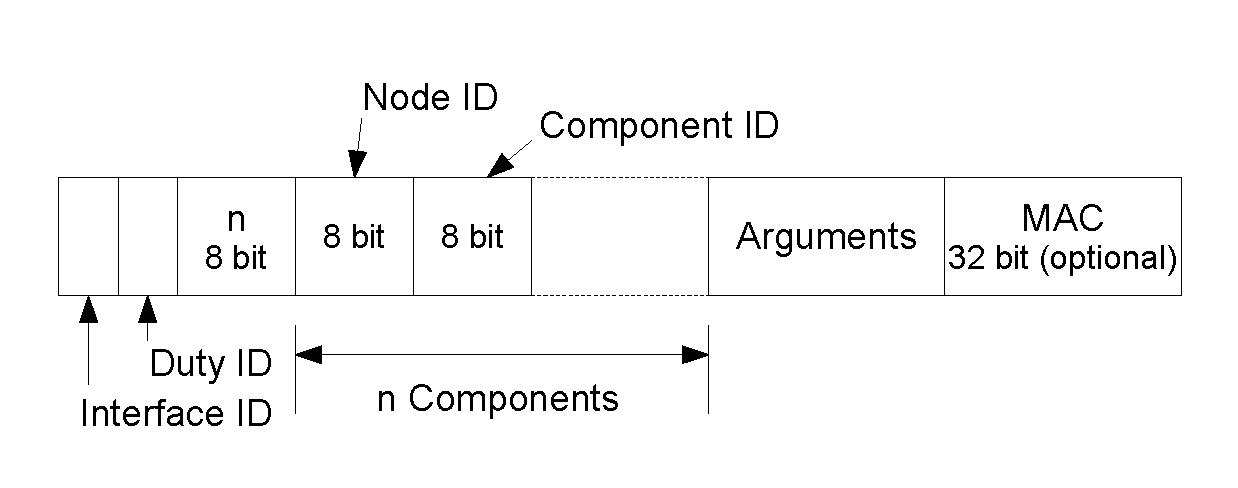
\includegraphics[scale=0.43]{packet}
  \caption{SpartanRPC data packet format.}
  \label{fig:packet}
\end{figure}

The SpartanRPC packet header can introduce significant overhead in some cases. In the current
version of Sprocket, $I$ and $D$ are packed as two four bit fields in a single byte. Each
intended destination is identified by a byte for $N$ and a byte for $C$. Finally an additional
byte is used to encode the header's size. This yields a total overhead of $2 + 2n$ bytes where
$n$ is the number of components intended to receive the packet. A special node ID of \code{0xFF}
is used to represent a SpartanRPC level broadcast. Thus in the special (and common) case where
all neighbor nodes are to process the remote call the overhead is exactly four bytes, leaving 12
bytes for duty parameters. If a parameterless duty is called, the maximum fan out supported by
our implementation is seven.

The limited field sizes used in the header put static restrictions on the system. Only 16 remote
interfaces per component can be used with at most 16 duties per interface. In addition, the
current version of Sprocket limits the network to at most 255 nodes with 256 remotely accessible
components per node.

\subsection{Skeleton Generation}

For each remote interface provided, Sprocket converts the duties in the component providing that
interface into nesC commands. Sprocket also generates a skeleton component for every remote
interface implementation. These skeletons are connected to the active message components in the
TinyOS library. Each time a duty message is received the skeleton checks the packet for
applicability. If the packet is not intended for the $(N, C, I)$ triple supported by the
skeleton or if $D$ is out of bounds for the interface, the packet is ignored. In the interest of
minimizing radio traffic, no error indication is returned.

If the packet is applicable, the skeleton unmarshalls the message, stores the duty arguments in
skeleton-local variables, and posts a task that implements the duty. For each duty in the
provided interface, Sprocket generates a trivial task in the skeleton that simply calls the
converted duty. For example:
\begin{Verbatim}
// 'value' written when packet unmarshalled.
uint8_t value;
task void setLeds()
    { call Blink.setLeds(value); }
\end{Verbatim}
\vspace{0.3em}

Thus the task-like semantics of duties are ultimately implemented in terms of ordinary nesC
tasks.

\subsection{Stub Generation}

On the RPC client side, Sprocket converts each duty posting into a command in a stub component
generated by Sprocket. That command first calls the \code{elements} command in the component
manager to obtain the list of target components. It then prepares a SpartanRPC data packet by
marshalling the duty arguments. Finally it broadcasts the packet to all neighboring nodes using
the TinyOS active message library. Recipients discern packets intended for them via packet
identifiers as described above.

Sprocket converts dynamic wires into static wiring that connects the posting component to the
generated stub. The stub is connected to the component manager associated with the dynamic
wiring. For example, a dynamic wire such as:
\begin{Verbatim}
ClientC.LEDControl ->
    [RemoteSelectorC].LEDControl;
\end{Verbatim}
is converted converted into the configuration as follows:
\begin{Verbatim}
components Spkt__1;
ClientC.LEDControl -> Spkt__1;
Spkt__1.ComponentManager -> RemoteSelectorC;
Spkt__1.Packet    -> AMSenderC;
Spkt__1.AMPacket  -> AMSenderC;
Spkt__1.AMControl -> ActiveMessageC;
Spkt__1.AMSend    -> AMSenderC;
\end{Verbatim}

The \code{Spkt\_\_1} component is the Sprocket generated stub.

\subsection{Security}

When capability-based security is used, Sprocket consults a configuration file that maps
capabilities to keys. To activate a capability over a dynamic wire, the Sprocket generated stub
computes a MAC that covers the SpartanRPC header and marshalled duty arguments. In the current
implementation this MAC is computed using the AES encryption algorithm in CBC mode with an
initialization vector of zero. Because SpartanRPC packets are currently limited to 16 bytes,
only a single AES encryption is necessary to compute the MAC. The first four bytes of the
resulting cipher text is used as the MAC value. While a MAC of only 32 bits would not normally
be considered secure, wireless sensor networks generate data so slowly that attacking even such
a short MAC is not considered feasible \cite{karlog-tinysec-2004,luk-minisec-2007}. Our MAC
computation is simplistic, but we feel it is adequate to demonstrate a proof of concept.

For components providing a secure remote interface, the generated skeleton incorporates a MAC
authentication procedure under the required key as declared in the component specification. The
usual checks of interface ID and component ID are done first so as to avoid a costly MAC
computation in the case where the received packet is not actually intended for the skeleton.
Only when the other applicability checks succeed is the MAC checked. The duty invocation is
ignored if the MAC check fails.



% ------------------------------
% Appendix and related materials
% ------------------------------

\bibliographystyle{plain}
\hbadness=10000 % Don't tell us how bad the bibliography really looks. We do not want to know.
{
\small
\bibliography{../../../BibTeX/references-WSN}
}

\end{document}

